\section{Results}
Unblinding the signal regions did not reveal any evidence for high muon-multiplicity events in the 2010 CMS dataset.  Exact numbers of events in each topology are given in Table~\ref{tab:results}.
The only region with a large number of events is (a-1), the
high-momentum dimuon region (which was expected from
Fig.~\ref{fig:support_bbbarcut_limits}(a)).  An incisive test of this
signal region is given in the fit results, below.  The (a-2) topology
includes one event (see event display in Appendix~\ref{sec:appendix_event_displays}), but the two dimuons in
this event are not consistent with a single mass.  Similarly, the
(b-1) region includes 9 events (see sample event display in
Appendix~\ref{sec:appendix_event_displays}), but none of these are
consistent with a single $m_1$ mass.

\begin{table}[tbh]
\caption{Number of observed events in each signal category.  For regions
  with $N \ge 2$ dimuons, the number of events is shown both for the entire category 
  as well as for the 5-$\sigma(m)$ signal region near the $N$-dimensional diagonal ($\sigma(m,p_T) = (0.026 + 0.0065\, m$~GeV/$c^2$ for (a-2) and $\sigma(m,p_T) = (0.026 + 0.013\, m$~GeV/$c^2$ for (b-1)). \label{tab:results}}
\vspace{0.1 cm}
\begin{tabular}{c l | c c}
\hline\hline Signal region & Description & Number of events & on diagonal \\\hline
(a-1) & $N_{\mu-jet} = 1$, $N_{\mu} = 2$, $p_T > 80$~GeV/$c$ & 145 & --- \\
& $2m_\mu < m < 0.25$~GeV/$c^2$ & 4 & --- \\
& $0.25 < m < 5$~GeV/$c^2$ & 130 & --- \\
& $5 < m < 9$~GeV/$c^2$ & 11 & --- \\
(a-2) & $N_{\mu-jet} = 1$, $N_{\mu} = 4$ (opp.\ sign pairs) & 1 & 0 \\
(a-3) & $N_{\mu-jet} = 1$, $N_{\mu} > 4$ & 0 & 0 \\
(b-1) & $N_{\mu-jet} = 2$, $N_{\mu} = 2$ in each & 9 & 0 \\
(b-2) & $N_{\mu-jet} = 2$, $N_{\mu} > 2$ in at least one & 0 & 0 \\
(c-1) & $N_{\mu-jet} \ge 3$ & 0 & 0 \\\hline\hline
\end{tabular}
\vspace{0.1 cm}
\end{table}

No high muon-multiplicity events
were observed in any of other signal topologies. Figure~\ref{fig:signalregion_events} shows
the distributions for regions (b-1), (a-1), and (a-2) with the background-only fit overlaid 
with the data.  We also show the invariant mass of the four muons for the single event in the \mbox{(a-2)} category 
found in the off-diagonal part of the region sets the upper limit on the possible production of 
$h_D \to \gamma_D \gamma_D$ in the special scenario where $m(h_D)<2 m(\gamma_D)$ leading to 
the off-shell production of $\gamma_D$. 

\begin{figure}[tbh]
\centering
\begin{tabular}{cc}
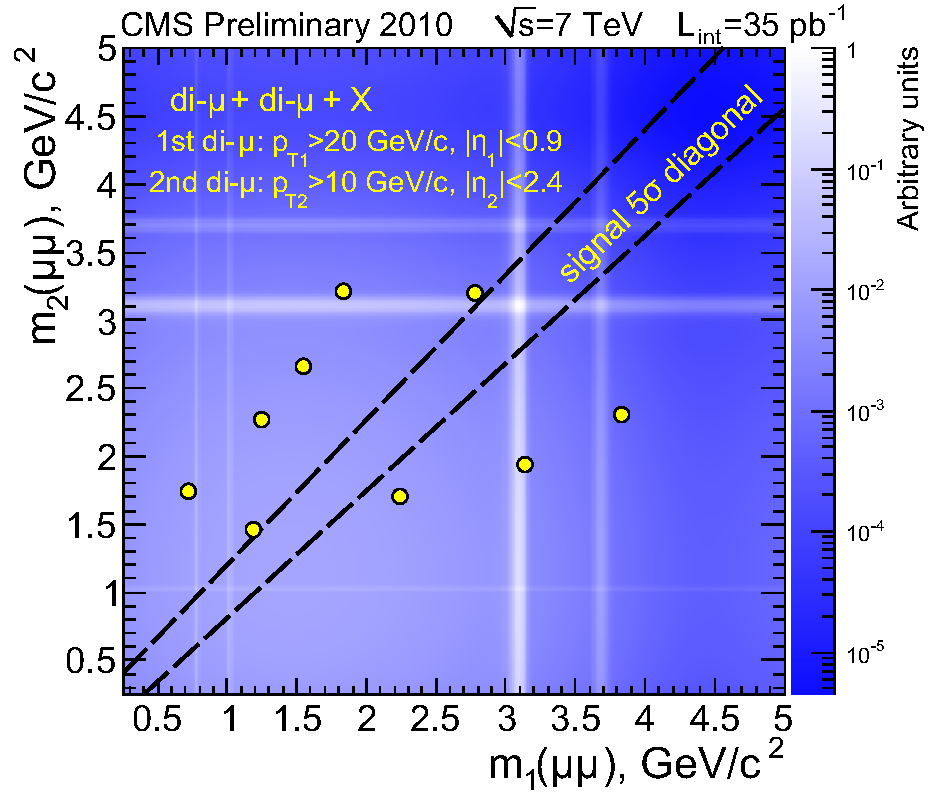
\includegraphics[width=0.4\linewidth]{PLOTS/sig_data_bg_b1.pdf} &
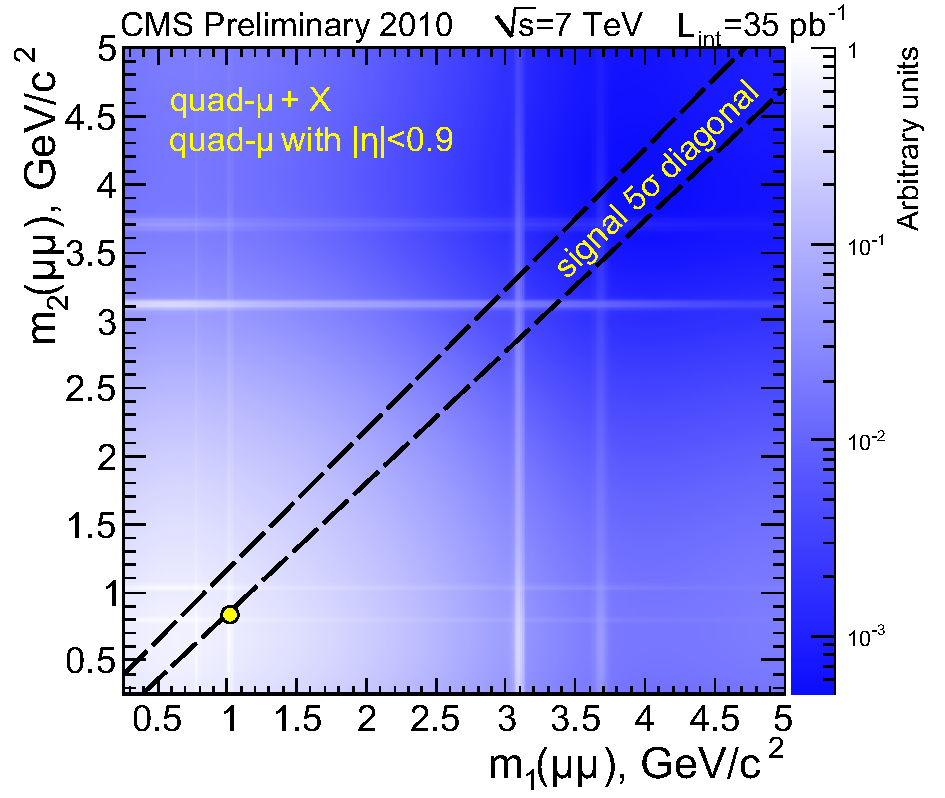
\includegraphics[width=0.4\linewidth]{PLOTS/sig_data_bg_a2.pdf} \\
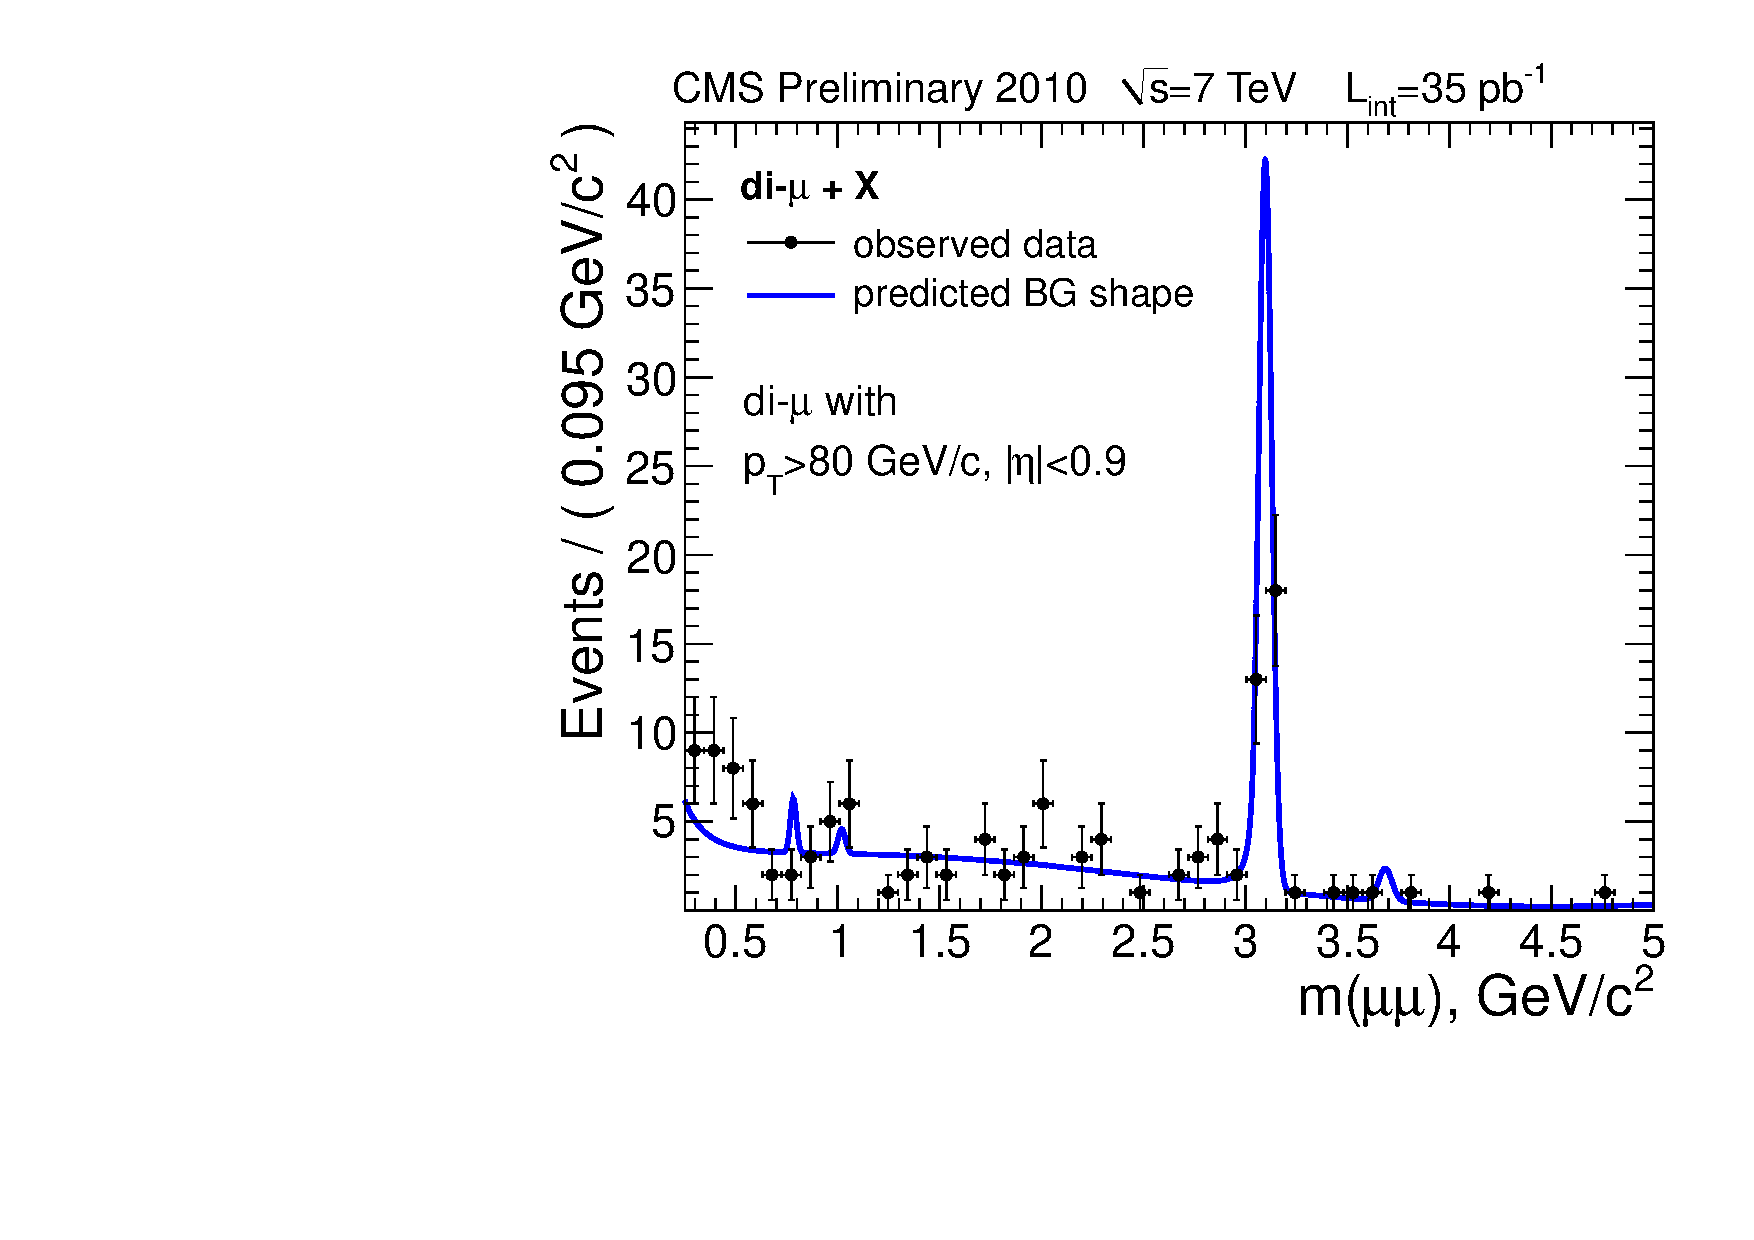
\includegraphics[width=0.4\linewidth]{PLOTS/sig_data_bg_a1.pdf} & 
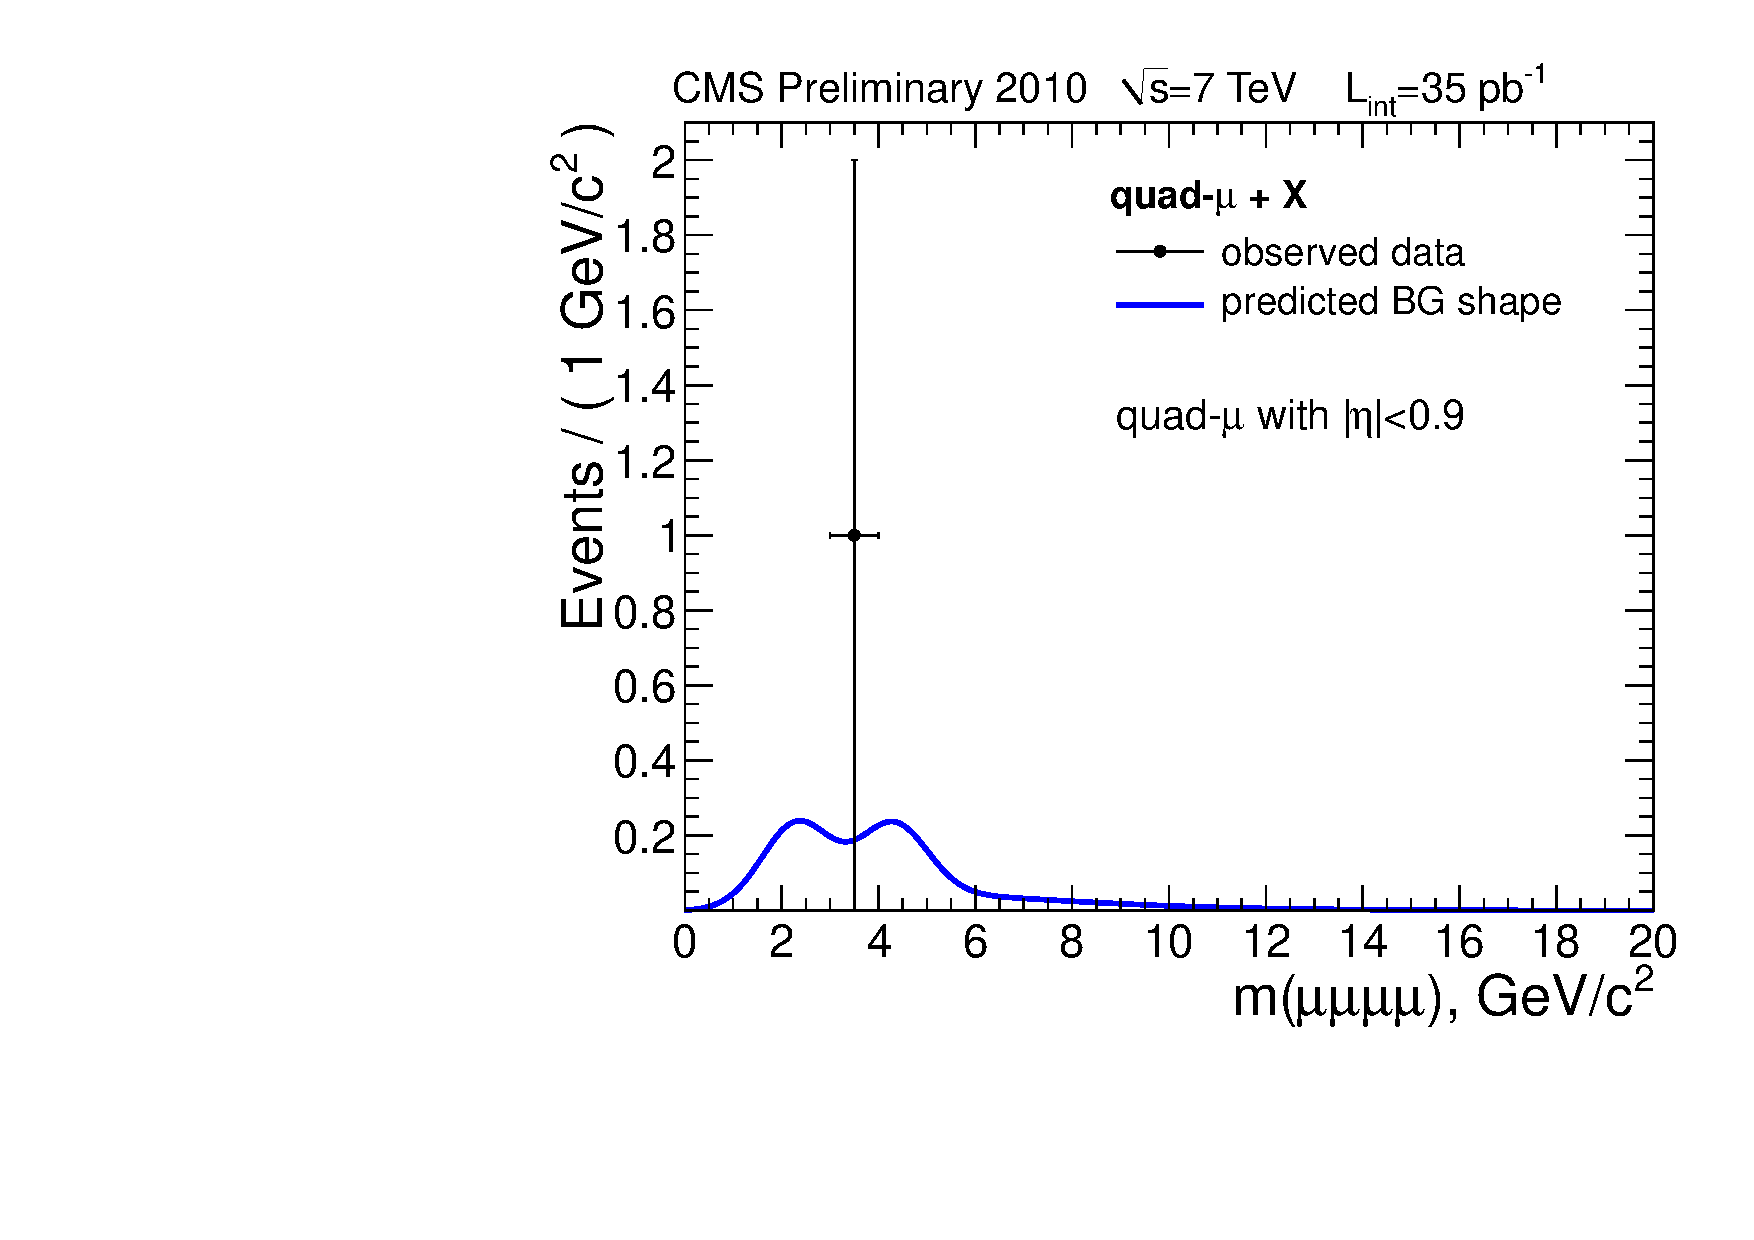
\includegraphics[width=0.4\linewidth]{PLOTS/sig_data_bg_a2_inv.pdf}\\
\end{tabular}
\caption{2D and 1D distributions of events in data and expected backgrounds in signal categories: (a): ``double dimuon'' region (b-1), (b): the ``quadmuon'' region category (a-2), (c): ``single dimuon'' region (a-1), (d): (b): the invariant mass of the four muons for the single event in the``quadmuon+X'' category found in the off-diagonal part of the region sets the upper limit on the possible production of $h_D \to \gamma_D \gamma_D$ in the special scenario where $m(h_D)<2 m(\gamma_D)$ leading to the off-shell production of $\gamma_D$. None of the events in the signal categories have invariant masses of the dimuons consistent with one another, which would indicate presence of signal. The dashed lines indicate signal regions for 2D categories (those are five standard deviations from the diagonal in detector resolution). No events were observed in any of the high dimuon-multiplicity regions (a-3), (b-2), or (c-1). \label{fig:signalregion_events}}
\end{figure}

\subsection{Model Independent Results}
\begin{figure}[tbh]
\centering
\begin{tabular}{c}
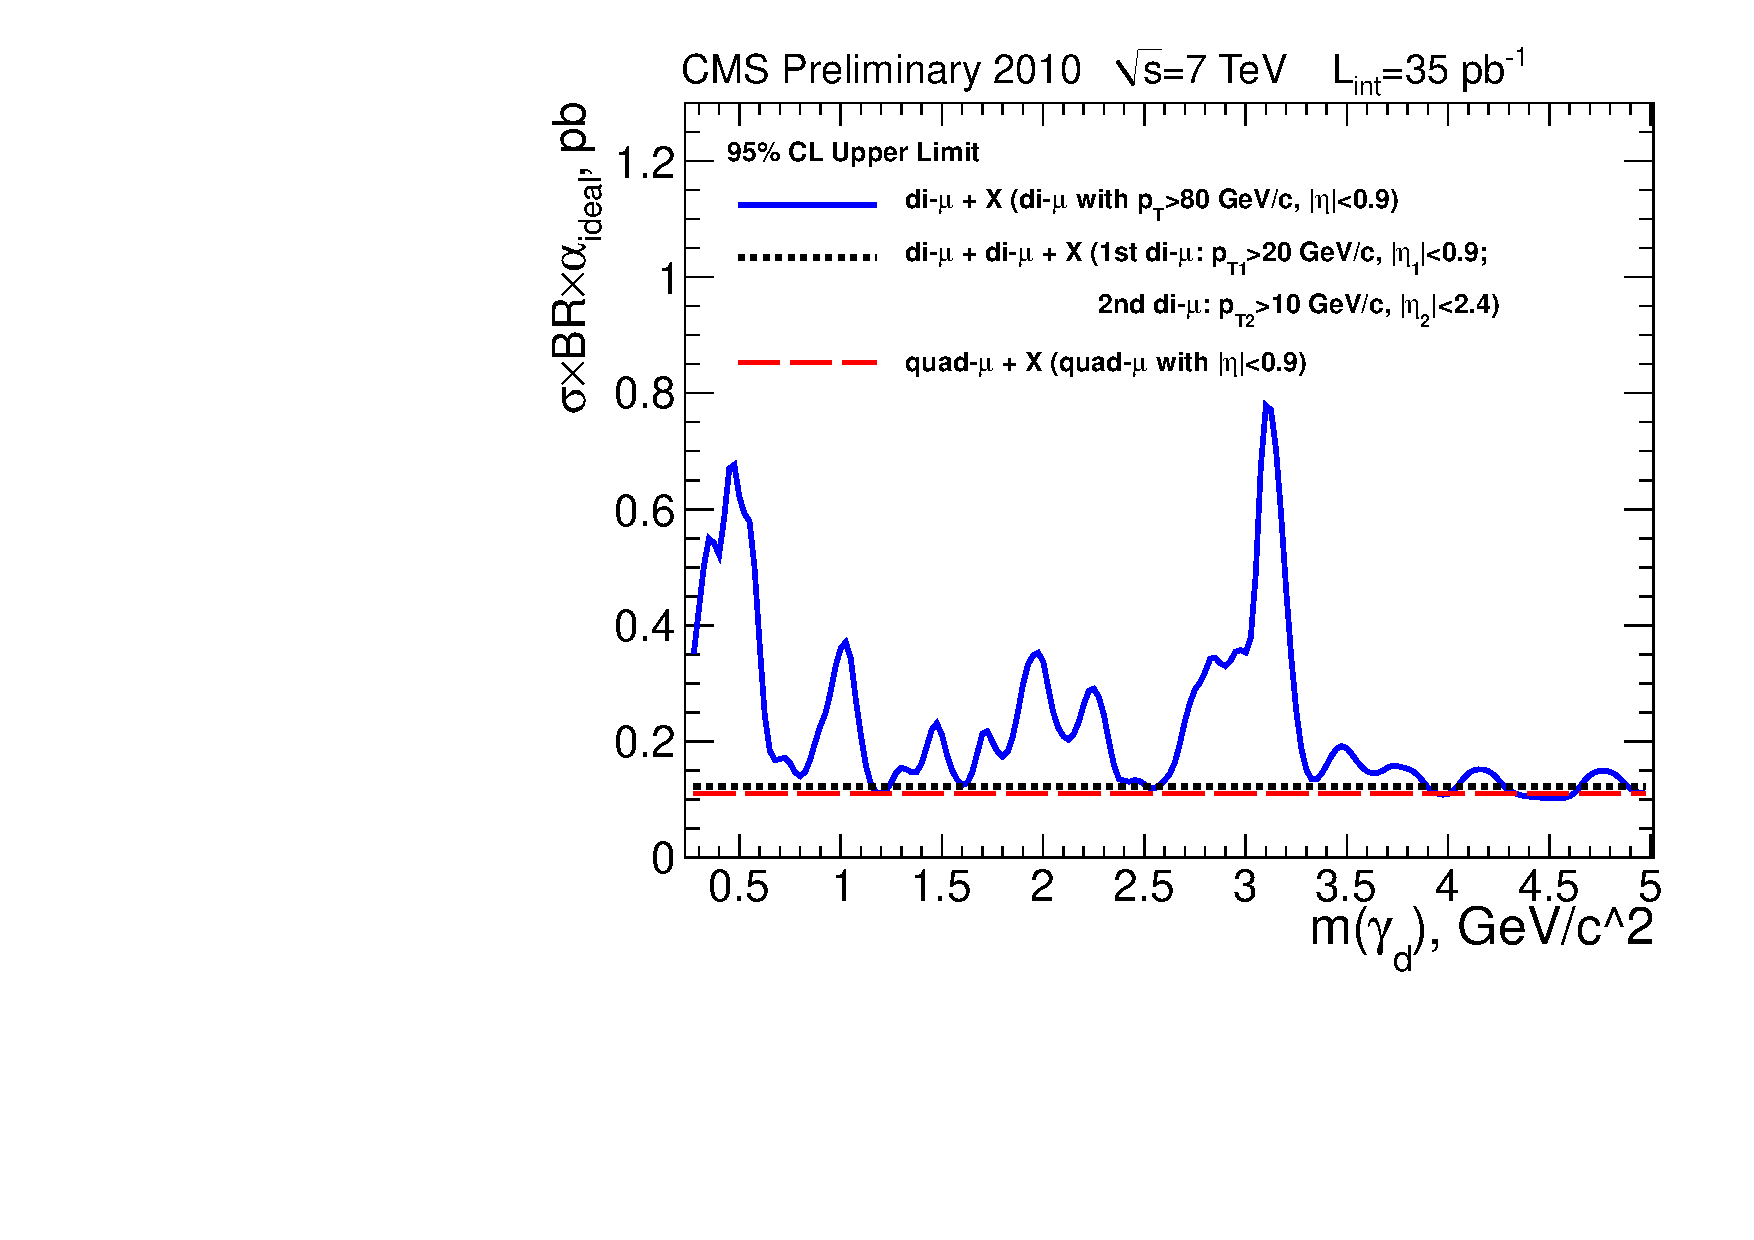
\includegraphics[width=0.65\linewidth]{PLOTS/ul__model_indep_sys.pdf} \\
\end{tabular}
\caption{95\% C.L. limits on production cross-section for three topologies: ``single dimuon'' (a-1),  ``two dimuons'' (b-1) and ``quadmuon+X'' (all others). In the absence of signal events for the two latter topologies, the limits for regions correspond to three signal events corrected for the experimental efficiency of reconstructing this particular topology in the data given that the event was reconstructed in that topology at the generator level. \label{fig:signalregion_limits}}
\end{figure}

Given no observed excess of data consistent with the properties of the signal of new physics, we set 95\% C.L. upper limits on the production rate of the new physics events. To simplify future interpretation of our results, we choose to present these limits as $\sigma(pp \to X) \times B(X \to N a_{\mbox{\scriptsize dark}}+M h_{\mbox{\scriptsize dark}}) \times \alpha_{\mbox{\scriptsize gen}}$, where $\alpha_{\mbox{\scriptsize gen}}$ is the ideal detector (generator level but with geometric and kinematic selections on muon $p_T$ and $\eta$) acceptance for the events of the topology in question. Because no events were observed in any of the high dimuon-multiplicity regions (a-3), (b-2), and (c-1), we combine them into a single region.  To be conservative, in cases when experimental acceptances for lower multiplicity dimuon regions in complex cascade models get an additional enhancement due to higher-multiplicity signatures with some of the dimuons not reconstructed in the fiducial volume, the experimental acceptance is taken to be generator level acceptance multiplied by corresponding efficiencies of reconstruction and triggering (and so can never be greater than generator level acceptance). In some models with large number of final state dimuons, these enhancements can be fairly substantial, so this approach can be very conservative for such models. However, for the results to remain being applicable to a wide range of models, this seems like the only reasonable solution. In this case $\epsilon_\alpha$ in Eq.~(\ref{likelihood_final}) is the experimental efficiency of reconstructing a particular topology in the data given that the event was reconstructed in that same topology at the generator level. For systematics, the parameters used in the fit are listed in Table~\ref{tab:syst_params_model_indep} along with the description of the priors used in the fit.

\begin{table}[tbh]
\caption{List of systematic uncertainties used for setting model-independent limits. (*) $\alpha$ and $n$ in Crystal Ball are strongly correlated, the correlation coefficient used was $-0.9$ based on MC studies of $J/\psi$ and $\psi^\prime$, and cross-checked with data. Acceptance uncertainties are for $\alpha_{rec}/\alpha_{ideal}$ and includes the systematic uncertainties in the knowledge of efficiencies as well as a separate uncertainty to account for variations in the tracking efficiency itself with $p_T^{\mu-jet}$ and $m(\mu\mu)$. For the latter we assume that the bulk of the $p_T^{\mu-jet}$ distribution is below 400 GeV/c and the mean $p_T^{\mu-jet}\leq 250$ GeV/c. For higher momentum lepton jets, the uncertainties will need to be increased to account for the decrease in tracking efficiency.  \label{tab:syst_params_model_indep}}
\begin{center}
\begin{tabular}{| p{0.25\linewidth} | ccc|p{0.25\linewidth}|}
\hline\hline 
Systematic & \multicolumn{3}{|l|}{Region}              & Prior \\\hline
                  & (a-1) & (a-2) & (b-1) & \\hline
Luminosity  & 4\%  & 4\% & 4\% & Log-normal \\
\multicolumn{3}{|l|}{Acceptance parameters:} \\\hline
$\alpha_{reco}/\alpha_{ideal}$ & $94.7 \pm 0.1\%$ & $79.3 \pm 0.3\%$ & $89.8 \pm 0.2\%$ & -- \\\hline 
$\alpha_{EB}/\alpha_{BB}$ & -- & -- & $0.55 \pm 0.05$ & Log-normal \\
\multicolumn{5}{|l|}{Acceptance uncertainties:} \\\hline
Muon eff. incl. trigger & 1\%& 2.3\%& 4\%  & Log-normal \\
Tracking eff. uncertainty vs $m(\mu\mu)$ & 2-5\% & 2\% & 4-10\%  & Log-normal \\
Tracking eff. variation vs $p_T^{\mu-jet}$ & 20\% & 7\% & 35\%    &  Log-normal\\
\hline
\multicolumn{5}{|l|}{Signal Shape (Crystal Ball parameters):} \\\hline
$\sigma_0^B$ & \multicolumn{3}{|l|}{$0.00675\pm 0.00325$} & Log-normal \\
$\sigma_0^E$ & \multicolumn{3}{|l|}{$0.0075 \pm 0.0040$} & Log-normal \\
slope$^B_{\sigma}$  & \multicolumn{3}{|l|}{0.0070} &--\\
slope$^E_{\sigma}$  & \multicolumn{3}{|l|}{0.0140} & --\\
$\alpha$ & \multicolumn{3}{|l|}{$1.8 \pm 0.16$} & bi-variate gaussian$^*$ \\
$n$ & \multicolumn{3}{|l|}{$2.0 \pm 0.6$} & bi-variate gaussian$^*$ \\
\hline
\multicolumn{5}{|l|}{Background Shapes:} \\\hline
$\vec{p}_{BG}$ & \multicolumn{3}{|l|}{} & Actual multi-dim posteriors from the fits \\
\hline\hline 
\end{tabular}
\end{center}
\end{table}


\subsection{Limits on Benchmark Models}

For model dependent results, we use reconstruction level acceptances calculated using the simulation for each of the signal regions. The likelihood function is calculated for each of the regions and the sensitivity of the various channels was combined at the level of likelihoods prior to integrating over the nuisance parameters to ensure that the correlated systematics effects are correctly accounted for. In addition to the systematic uncertainties listed for the model-independent case, the model-dependent limits take into account the 3\% uncertainty in the acceptance due to PDF uncertainties (obtained using CTEQ6.6 and comparing the default parameterization CTEQ6L with the NNPDF2.0 and MSTW-2008). Additionally, the higher muon multiplicity category is taken into account in the acceptance estimation. Because in this case the muon momentum spectrum is known in each case and the limits are set for specific mass points, the variation of efficiencies to account for the unknown mass and $p_T$ spectrum is not used.

\begin{table}[tbh]
\caption{List of systematic uncertainties used for setting model-dependent limits. Signal shape parameters
are the same as in the model-independent case. Uncertainties assume mean $p_T^{\mu-jet}<200$ GeV/c$^2$,
which is true for all models used. \label{tab:syst_params_model_dependent}}
\begin{center}
\begin{tabular}{| l | cccc|l|}
\hline\hline 
Systematic & \multicolumn{4}{|l|}{Region}              & Prior \\\hline
                  & (a-1) & (a-2) & (b-1) & others & \\hline
Luminosity  & 4\%  & 4\% & 4\%  & 4\%     & Log-normal \\
PDF (accept.) & 3\%  & 3\% & 3\%  & 3\%      & Log-normal \\
Muon eff. incl. trigger & 1\%& 2.3\%& 4\% & 4\% & Log-normal \\\hline
\multicolumn{4}{|l|}{Tracking eff. uncertainties}  \\
$m(\mu\mu)=0.25$ GeV/c$^2$   & 2\% & 2\% & 4\%   & 4\%   & Log-normal \\
$m(\mu\mu)=0.50$ GeV/c$^2$   & 5\% & 2\% & 10\% & 10\%  & Log-normal \\
$m(\mu\mu)\geq1.0$ GeV/c$^2$ & 2\% & 2\% & 4\%  & 4\%   & Log-normal \\
\hline\hline 
\end{tabular}
\end{center}
\end{table}

As one example, we calculate the limit on the production cross section times branching ratio for dark SUSY models with dark fermion production. Acceptances for the two model variations, $B(\tilde{q} \to q (n_2 \to n_1 \gamma_D))=100$\% and $\tilde{q} \to q n_2 (\to n_1 h_{D} (\to 2 \gamma_{D}))=100$\%, with  sqark-squark and squark-gluino production the acceptance is shown in Tables~\ref{tab:all_squark2} and ~\ref{tab:all_squark4} for three choices of 
$B(\gamma_D \to \mu \mu)=$100, 50, and 33\%. Depending on the branching fractions and the model, the limit is dominated by different signal regions with the results shown in Figs.~\ref{fig:ulimit}(a) and (b). Note the weak dependence of the limit on squark mass, emphasizing the weak model-dependence of the 
results of this analysis. It is important as the branching fractions for squark decays to the dark sector fermions are not 100\%, e.g. due to a 
weaker coupling of the dark and visible sectors.

In the case of extra $\mathcal{U}(1)_{dark}$ model, Table~\ref{tab:all_u1} shows acceptances for each of the relevant regions for three 
choices of $B(\gamma_D \to \mu \mu)=$100, 50, and 33\%. Fig.~\ref{fig:ulimit}(c) shows the corresponding limit.

In the case of NMSSM, the sensitivity is dominated by the (b-1) category with the acceptance is of the order of 25\% (see Table~\ref{tab:all_nmssm}), which leads to a limit on the lightest CP-even NMSSM Higgs production rate $\sigma(pp \to h) B(h \to aa) B^2(a \to \mu \mu)\sim 0.4$ pb. Taking $B(a \to \mu \mu) \sim 20\%$ for $m(a)$ below $2 m_\tau$, this leads to an upper limit $\sigma(pp \to h) B(h \to aa) \sim 10$ pb. To set the limits and make a comparison with the Tevatron sensitivity, we follow the method used in~\cite{Belyaev:nmssm} and plot the density of model points consistent with LEP and the WMAP measurements in the plane of $B(h_1 \to a_1 a_1 \to 4 \mu)$ versus $\sigma (pp \to h_1)$ for $\sqrt{s}=7$ TeV. The experimental limits on such models from Tevatron and LHC exclude the upper right corner of this parameter space. Because exact limit for a particular model point depends on the acceptance for this specific point (via dependence on $m_h$ and $m_a$), experimental limits do not appear as strict lines in this plot. We therefore added the bands to show the range of limits that correspond to the range of acceptances for allowed models. Figure~\ref{fig:ulimit2} shows that with $L \sim 75$--$100$~pb$^{-1}$, the LHC sensitivity will surpass that of the Tevatron experiments and will significantly restrict the allowed 
parameter space with $L=1$ fb$^{-1}$.

\begin{figure}
\begin{center}
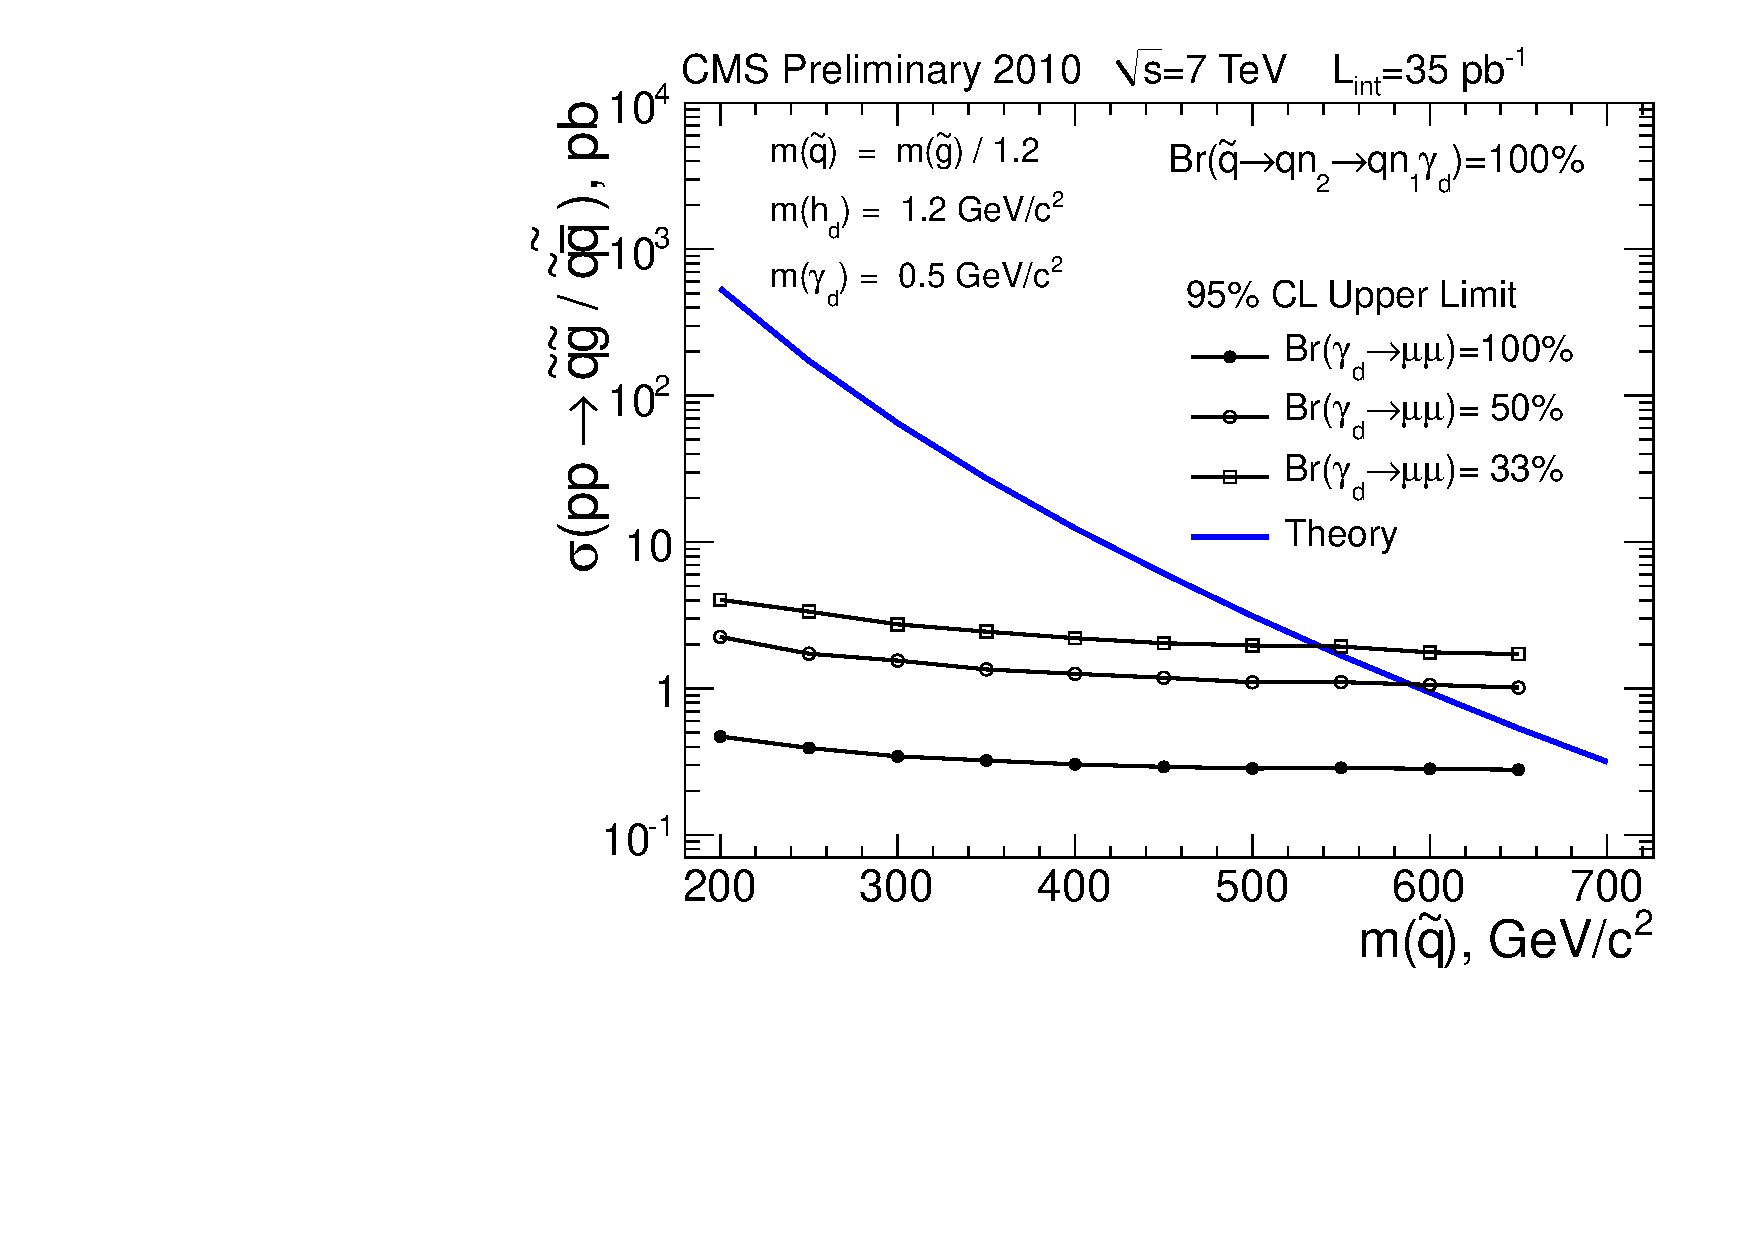
\includegraphics[width=0.45\linewidth]{PLOTS/ulimit_model0.pdf} \hfill
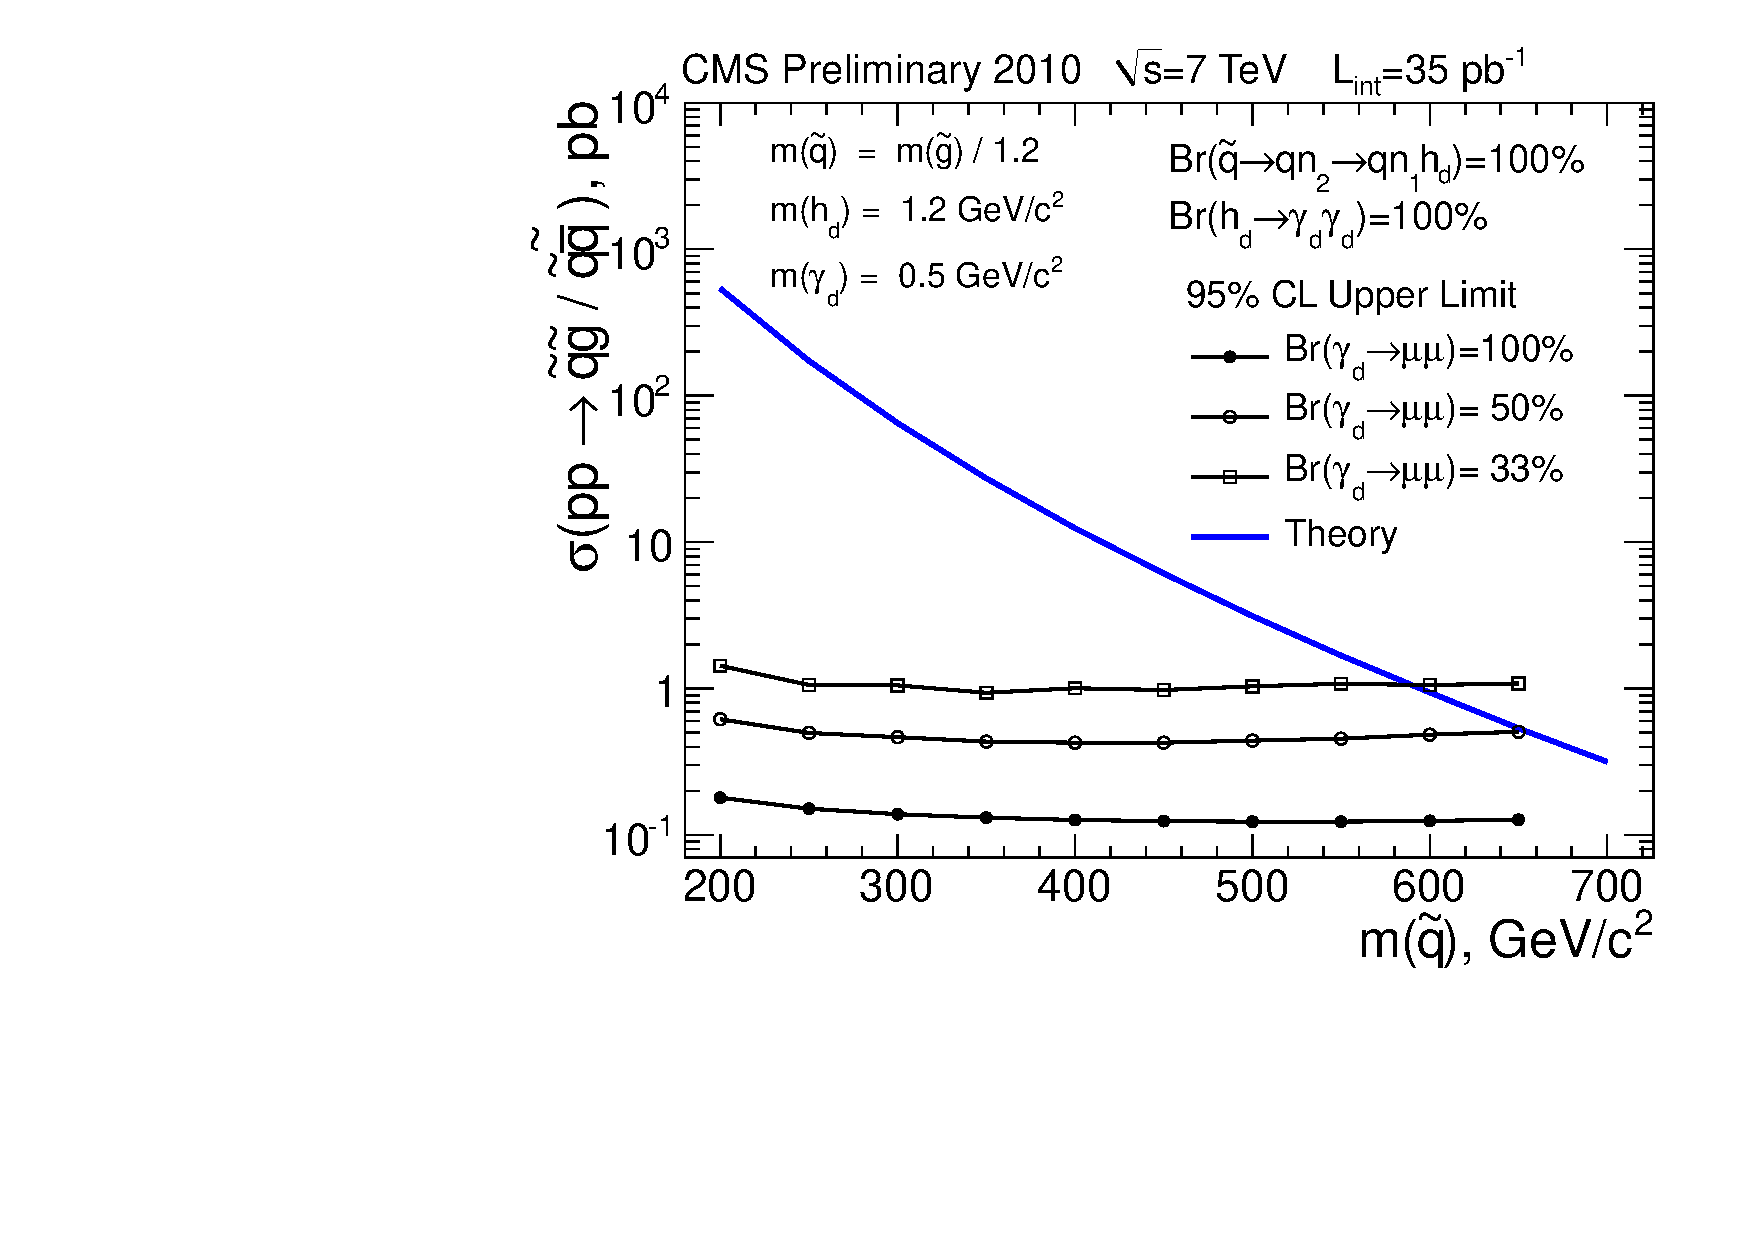
\includegraphics[width=0.45\linewidth]{PLOTS/ulimit_model1.pdf}
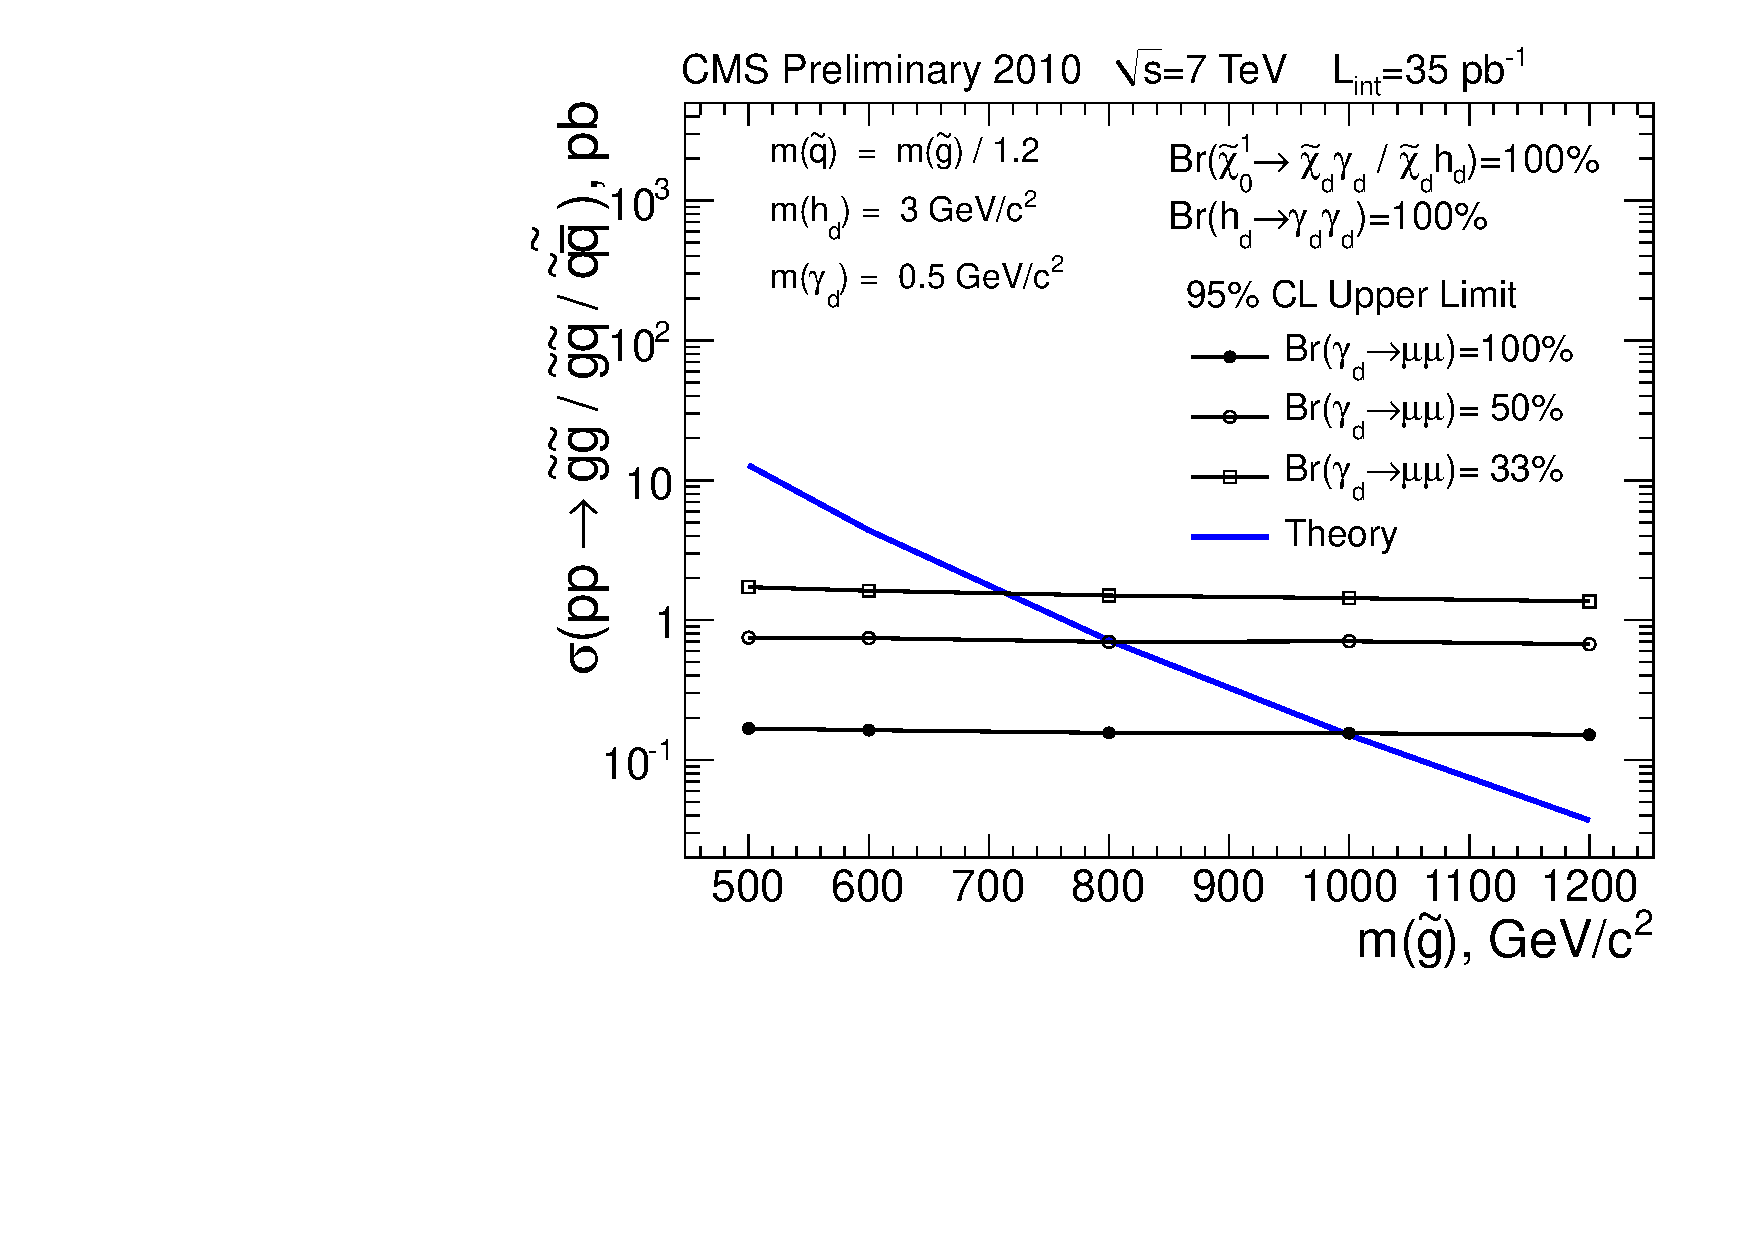
\includegraphics[width=0.45\linewidth]{PLOTS/ulimit_model_u1.pdf}
\end{center}
\caption{Limits on the Dark Fermion Cascades model and the Extra $U(1)_{dark}$ models described in Sections~\ref{sec:susy_with_dark_fermion_cascades}
and,~\ref{sec:susy_with_extra_u1} derived from the limits for each of the signal regions weighted with the model acceptance for each region.  
The $\gamma_{\mbox{\scriptsize dark}} \to \mu\mu$ branching fraction has a profound effect on the model acceptance and hence the final result. 
Note that the non-universality of squark masses can lead to decrease in the production cross sections. \label{fig:ulimit}}
\end{figure}

\begin{figure}
\begin{center}
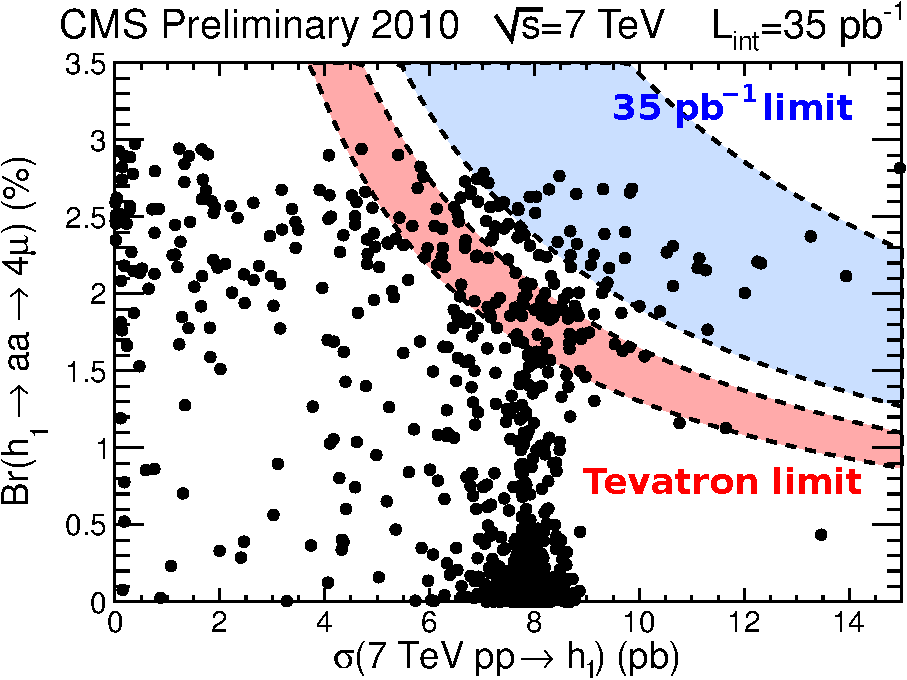
\includegraphics[width=0.48\linewidth]{PLOTS/limits_on_models_7tev.pdf}
\end{center}

\caption{Limits on the allowed NMSSM models consistent with LEP exclusions and the relic density measurements in the plane of $B(h_1 \to a_1 a_1 \to 4 \mu)$ versus $\sigma (pp \to h_1)$ for $\sqrt{s}=7$ TeV. The allowed models are shown as points and the experimental limits from Tevatron and LHC exclude the upper right corner of the parameter space. Because exact limits depend on the acceptance for each model point and therefore do not appear as strict lines, the bands show the range of limits that correspond to the range of acceptances for allowed models. The plot shows that with $L=1$~fb$^{-1}$ the LHC sensitivity will surpass that of the Tevatron experiments. \label{fig:ulimit2}}
\end{figure}

